 \chapter{Control of 2 Degree of Freedom}
\section{LQG Control Design}

The structure of this control scheme is the same as the 1 degree of freedom scenario and it is discussed in the previous chapter. In this section we only show the tuning and final results.\\

Obviously the state matrix includes also the second cart and we must take that into account when tuning the weights on $Q$, whilst the weight on the control input $R$ is again scalar. The final tuning was output of a trial and error approach which led to the matrices
\begin{equation}
\renewcommand{\arraystretch}{1}
	Q = 
	\begin{bmatrix}
		0 & 0 & 0 & 0 & 0 \\
		0 & 0 & 0 & 0 & 0 \\
		0 & 0 & 0.1 & 0 & 0 \\
		0 & 0 & 0 & 0 & 0 \\
		0 & 0 & 0 & 0 & 0 \\
	\end{bmatrix}
	\qquad
	R=1
\end{equation}
which only weights the position of the second cart (the one we want to control), being the state vector defined as $x = \left[ i,\, x_1,\, x_2,\, \dot{x}_1,\, \dot{x}_2 \right] $.\\

Since we are not including any integral action, we need to consider a compensator on the reference which can guarantee zero error at steady state. This gain is computed as the inverse of the dc gain of the controlled plant.

\begin{figure}[h]
\centering
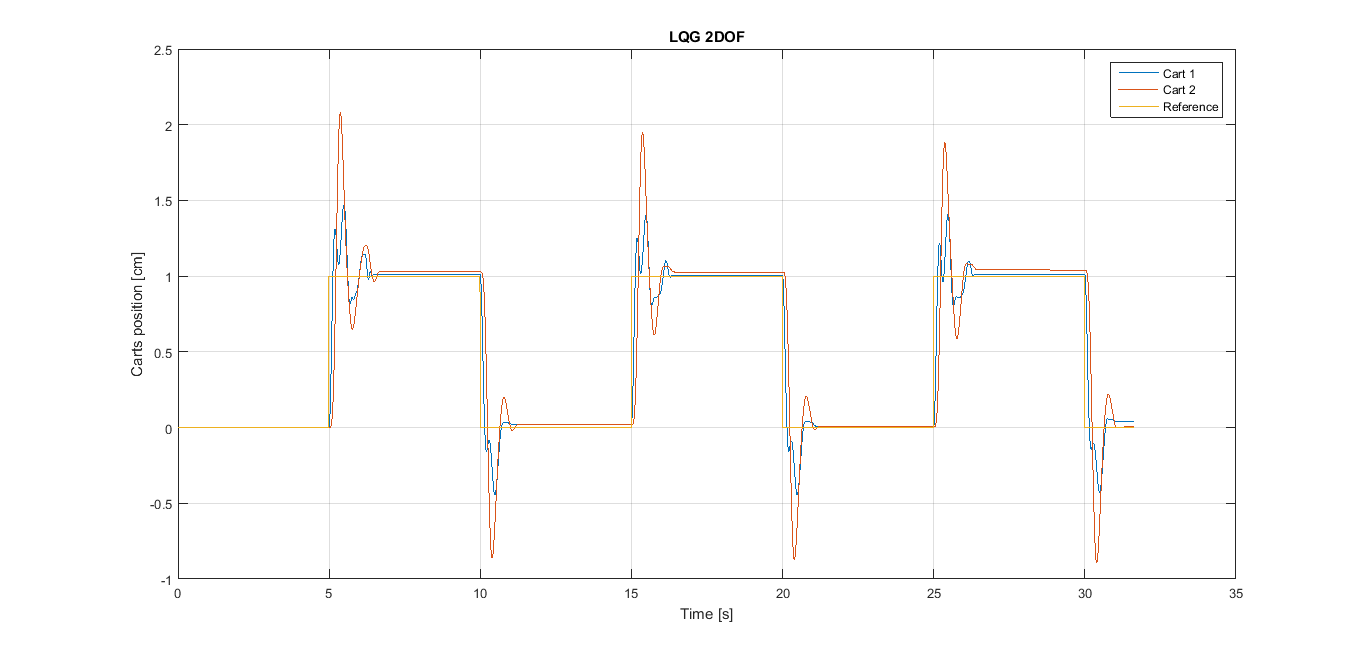
\includegraphics[width=0.5\linewidth]{img/lqg_2dof.png}
\caption{Openloop frequency response from the motor input to the position of the second cart in the case of low and medium springs employed.}
\label{fig:lqg2dof}
\end{figure}








\section{$H_\infty$ Control Design}
This control strategy gave good results for one degree of freedom, hence we choose it again to be implemented with two carts.\\

One important aspect is worth pointing out. The critical aspect in this scenario is which output feedback to the control input. If we feedback the first cart position, the control strategy won't be much different from the 1 degree of freedom, since the second cart is just equivalent to a heavier mass placed onto the first cart. This statement is confirmed by the fact that the controller designed in the previous chapter works fine in this scenario, meaning it is robust enough to uncertainties on the model.\\

Controlling the second output is instead more challenging since we have two springs in between the control action and the output to be controlled. In this case the controller must take into account both carts dynamics, and this is what we will discuss in this chapter.\\

%\begin{figure}[h]
%\centering
%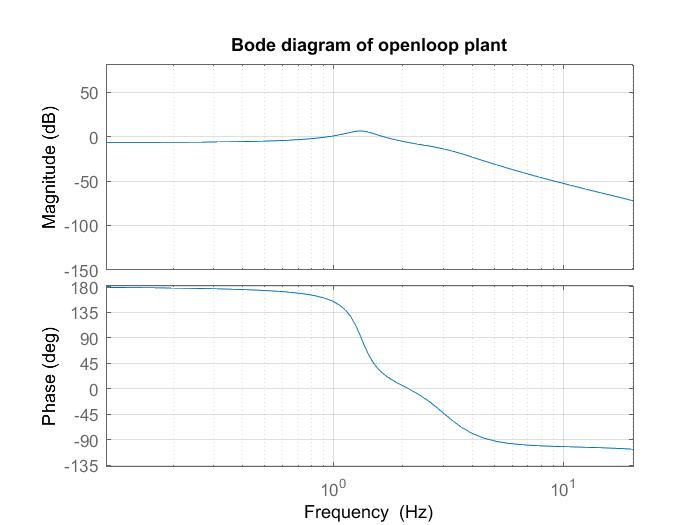
\includegraphics[width=0.5\linewidth]{img/bode_ol}
%\caption{Openloop frequency response from the motor input to the position of the second cart in the case of low and medium springs employed.}
%\label{fig:bodeol}
%\end{figure}

The plant, defined as the series of actuator followed by two carts is a 5th order system, where two complex conjugate poles come from the first cart, two from the second cart and one high frequency pole from the motor.\\

The controller design is exactly the same as the one presented in the previous chapter, hence we won't replicate it here but will only show the results.\\

As it possible to see, the current has some oscillations which perturb the whole system and gives very poor performance. The first attempt was to reduce te bandwidth of the controller but the output, although deprived from oscillations, resulted too slow (over two seconds in order to get to steady state) and therefore not acceptable.\\

We decided to make use of a Kalman filter in order to insert an inner loop controlling the current which consists in a simple integrator $R(s)=\frac{50}{s}$. The result showed an important boost in performance. The rising time is now satisfactory and the current does not show any oscillation.\\

\begin{figure}[h]
	\setlength{\abovecaptionskip}{-10pt}
	\setlength{\belowcaptionskip}{-10pt}
	\centering
	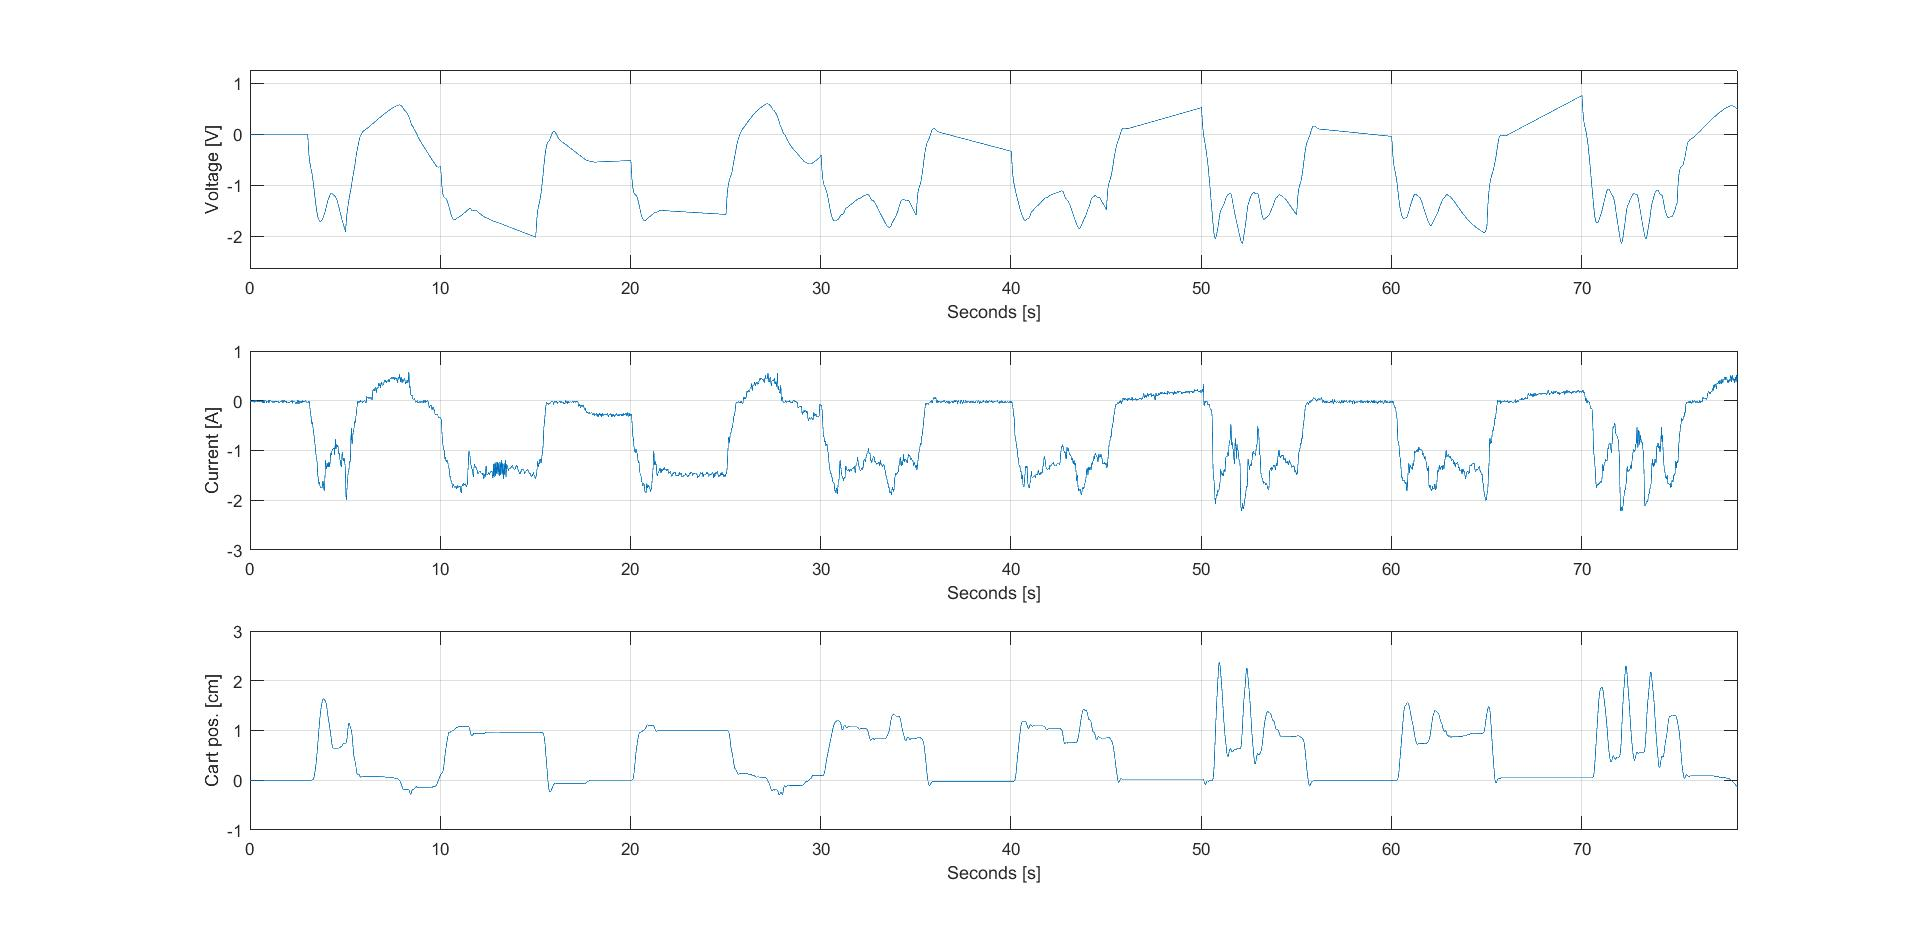
\includegraphics[width=0.7\linewidth]{img/hinf_nocurr}
	\caption{Response to a train of pulses when the current is not controlled. It is hard for the system to maintain the value at steady state.}
	\label{fig:hinfnocurr}
\end{figure}

\begin{figure}[h]
	\setlength{\abovecaptionskip}{-10pt}
	\setlength{\belowcaptionskip}{-10pt}	
	\centering
	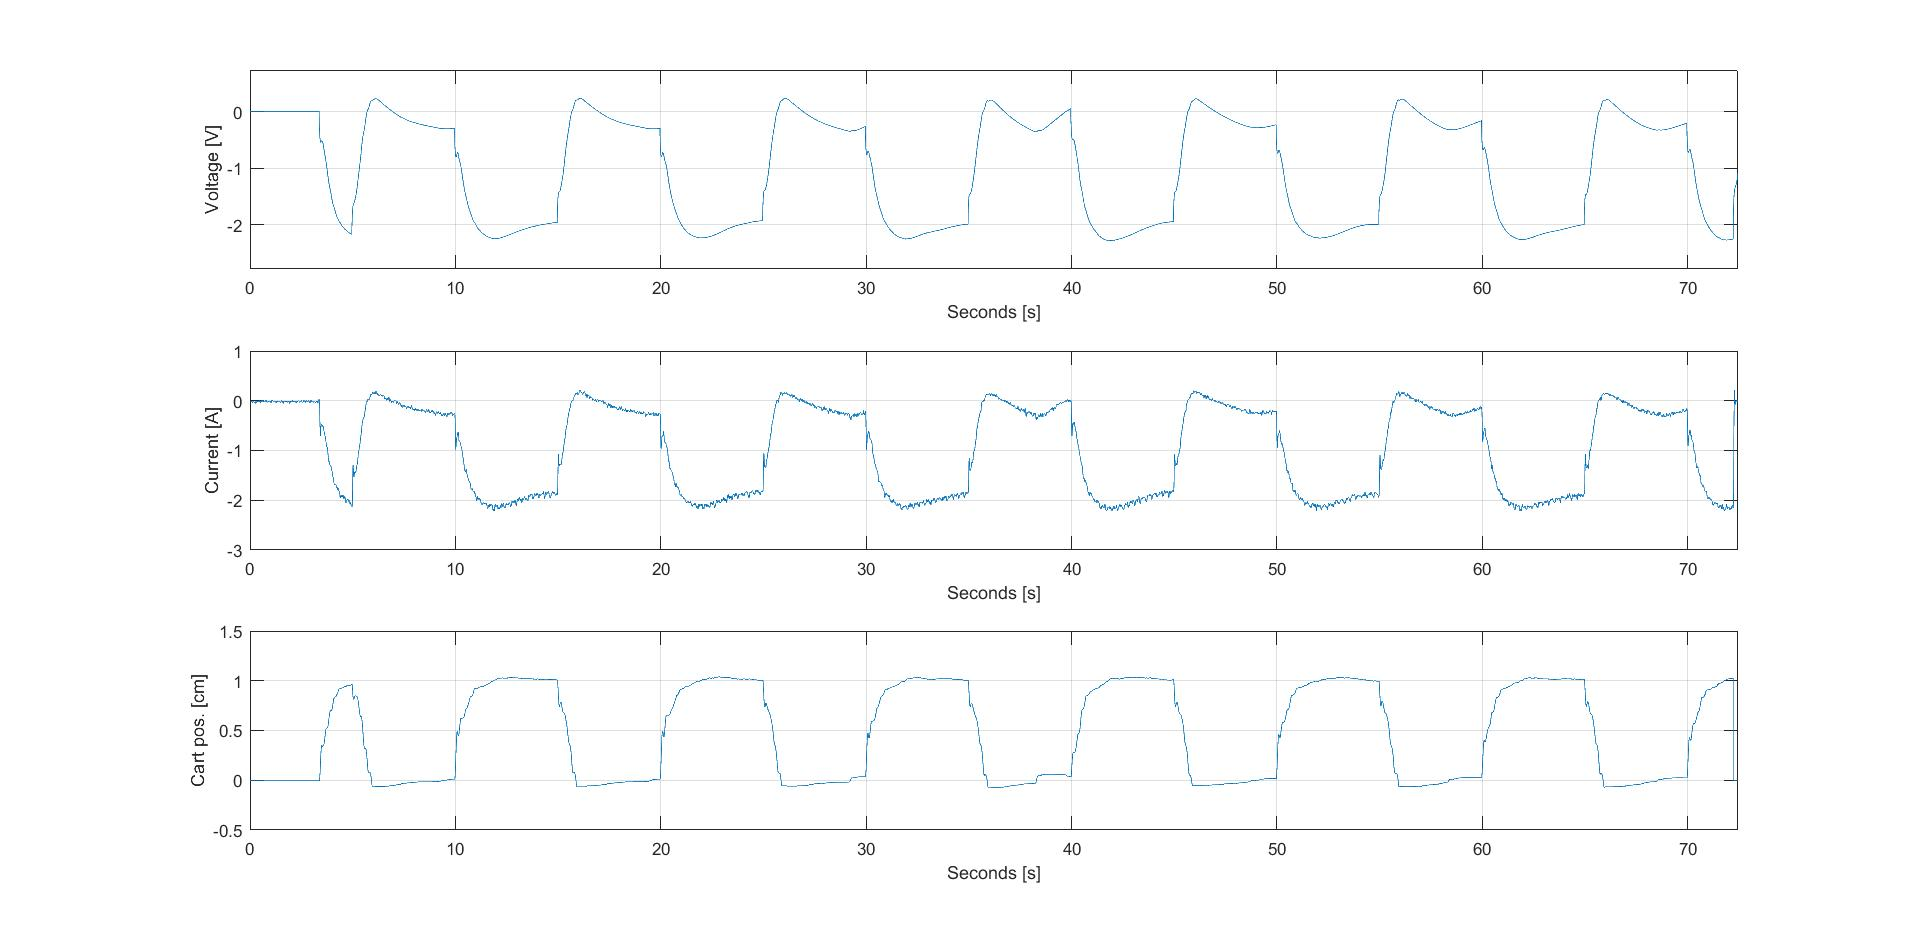
\includegraphics[width=0.7\linewidth]{img/hinf_curr}
	\caption{Response to a train of pulses when the current is controlled. Now the response is much smoother.}
	\label{fig:hinfnocurr}
\end{figure}

\begin{figure}[h]
	\setlength{\abovecaptionskip}{-10pt}
	\setlength{\belowcaptionskip}{-10pt}
	\centering
	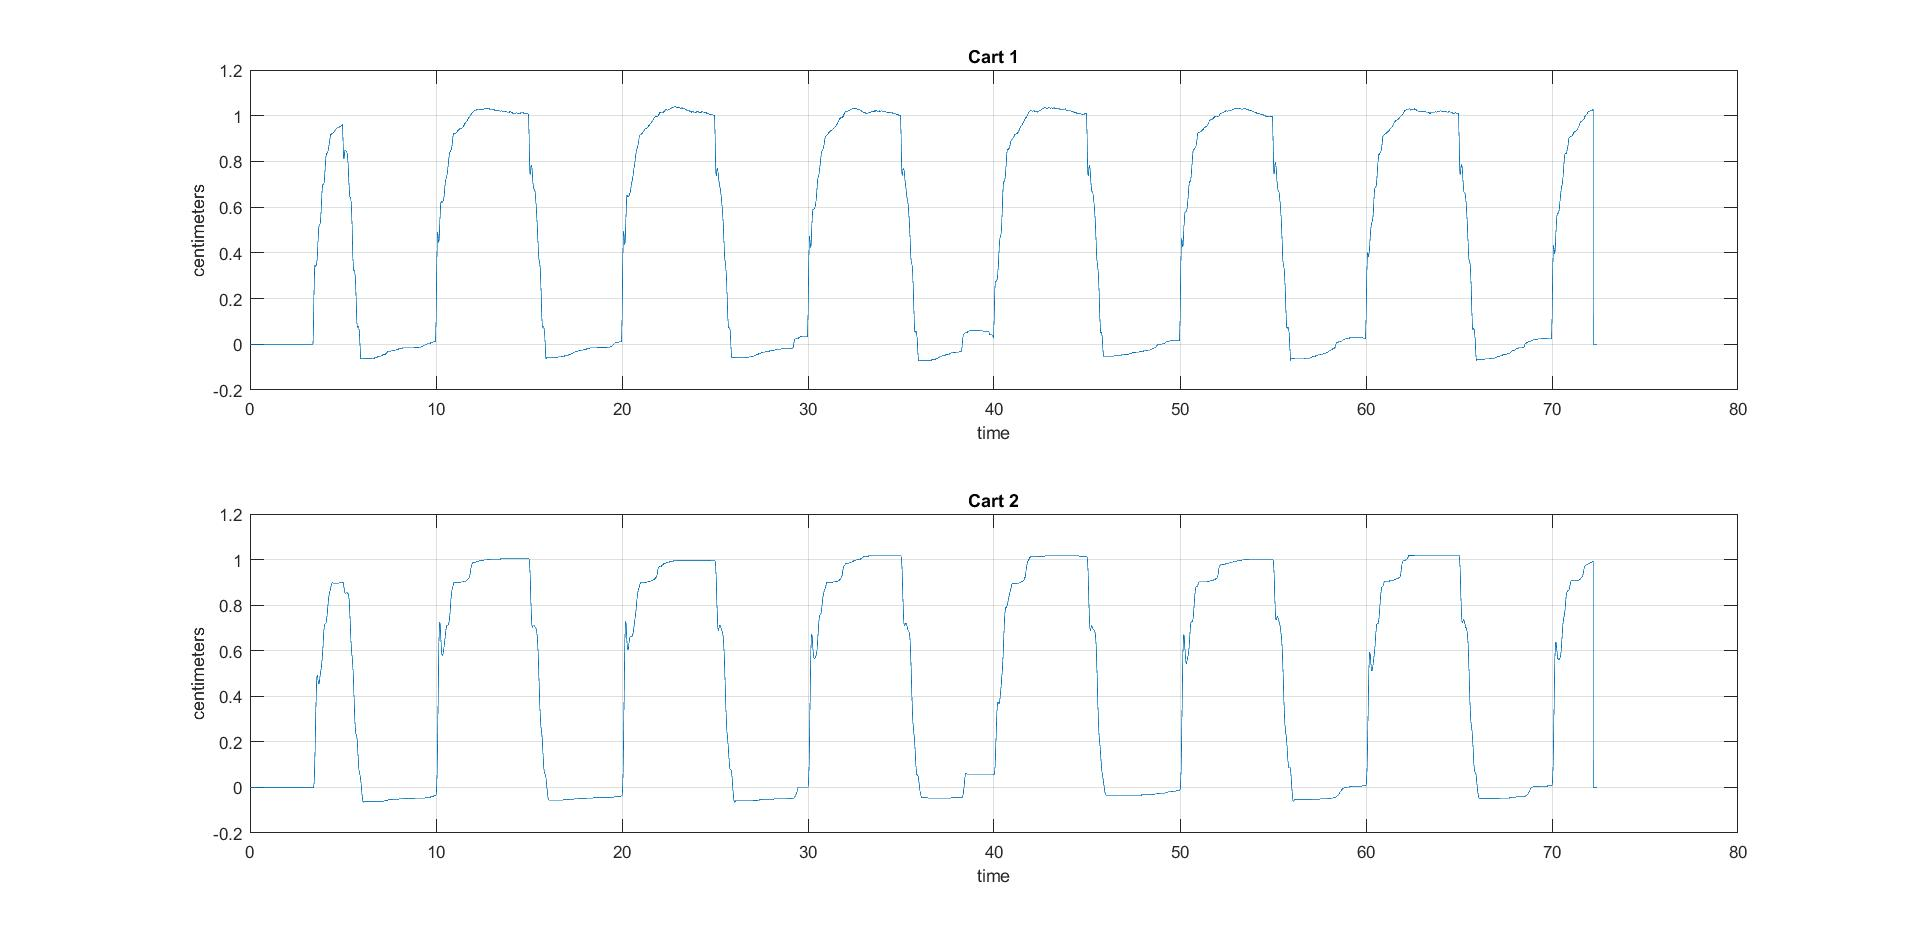
\includegraphics[width=0.7\linewidth]{img/hinf_response}
	\caption{Carts displacement over time due to a train of pulses. Both carts do not overshoot.}
	\label{fig:2dofcarts}
\end{figure}